\documentclass[12pt]{report}
\usepackage[spanish, activeacute]{babel}
\usepackage[top=2.75cm,bottom=2.50cm,left=3.00cm,right=2.50cm]{geometry}
\usepackage[utf8]{inputenc}  
\usepackage{enumerate}
\usepackage{graphicx}



\begin{document}
	\setlength{\topmargin}{-0.5in}
	\pagestyle{empty}
	\begin{center}
		\textbf{
			\vspace{-0.7em}
			ESCUELA SUPERIOR POLITÉCNICA DEL LITORAL
		}
		\line(1,0){380}\\		
		\scriptsize{FACULTAD DE INGENIERÍA EN ELECTRICIDAD Y COMPUTACIÓN}
	\end{center}

	\begin{center}
		\vspace{2.5em}
		\Huge{\textbf{\\PROYECTO FINAL}}
	\end{center}	

	\begin{center}
		\Huge{\textbf{\\Recopilación de Trabajos II Término 2012	\vspace{1em}}}
	\end{center}
	\begin{center}
		\Huge{\textbf{\\Ana Arias	\vspace{1em}}}
		\\ acarias@espol.edu.ec
	\end{center}
	\begin{center}
		\Huge{\textbf{\\Lenguajes de Programación\vspace{1em}}}
	\end{center}	
	\begin{center}
		\Huge{\textbf{\\Ing. Javier Tibau	\vspace{1em}}}
		\\ jtibau@espol.edu.ec
		\\ jtibau@fiec.espol.edu.ec
	\end{center}	



\chapter*{Agradecimientos}
\addcontentsline{toc}{chapter}{Agradecimientos} 
\markboth{AGRADECIMIENTOS}{AGRADECIMIENTOS} % encabezado 
 
Quiero agradecer a mis compañeros de grupo y compañeros del aula, ya que entre todos compartimos conocimientos y buenas experiencias.
También quiero agradecer a mi profesor de Lenguajes de Programación Ing. Javier Tibau por darnos todos los retos de este semestre.

\chapter*{Resumen} 
\addcontentsline{toc}{chapter}{Resumen} 
\markboth{RESUMEN}{RESUMEN} % encabezado

Este documento contiene las descripciones y experiencias de los proyectos realizados en la materia Lenguajes de Programación dirigida por el Ing. Javier Tibau.

\tableofcontents


%---------------------------------------------------------------------------------------------------------------------------------
%--------------------------------------------------------------GITHUB!------------------------------------------------------
%---------------------------------------------------------------------------------------------------------------------------------
\chapter{Herramienta GitHub\label{capitulouno}}

	\begin{center}
		\begingroup
			
\includegraphics[width=0.27\textwidth]{imagenes_usuario/git.png}
		\endgroup
	\end{center}


	\begingroup
		\large{
			\textbf{
			           \newline
			           \newline
				Experiencias y Anécdotas: GitHub
				\newline
				\newline
			}
		}
	\endgroup
Mi experiencia con GitHub ha sido buena, esta herramienta en verdad mejoró la comunicación en los trabajos con mi grupo; lo que más me agradó es que podemos estar actualizados con respecto a las modificaciones en los archivos que nos tocó hacer de forma grupal, y por lo tanto se evita el compartir documentos frecuentemente a través de otra herramienta y la creación de un sinfín de documentos que contienen en realidad lo mismo.
\newline
\newline	
Considero Github como una red social, ya que podemos estar conectados con nuestros compañeros y compartir información, y además de ser social, es seria ya que a partir de esta herramienta se pueden encontrar trabajos muy interesantes de distintas personas, dicho material puede ser muy útil.
\newline
\newline	
Con respecto a su uso, lo considero sencillo y mecánico; al principio es un poco difícil aprender cómo se utiliza pero después se vuelve costumbre ya que los procedimientos para subir archivos, para crear repositorios, para modificarlos es en realidad muy mecánico.
\newline
Esta herramienta es una buena opción para dar a conocer nuestros trabajos en internet, y seguramente la seguiré utilizando en el futuro.
\newline
\newline
Mi experiencia con Github a lo largo del semestre pasó de ser mala, a regular y finalmente a muy buena. Esto tiene mucho que ver por toda la practica que tuvimos que tener con esta herramienta, ya que la utilizamos en todos los proyectos.
El uso de la herramienta Github se facilitó mucho cuando empecé a utilizar su interfaz.
\newline
	\begin{center}
		\begingroup
			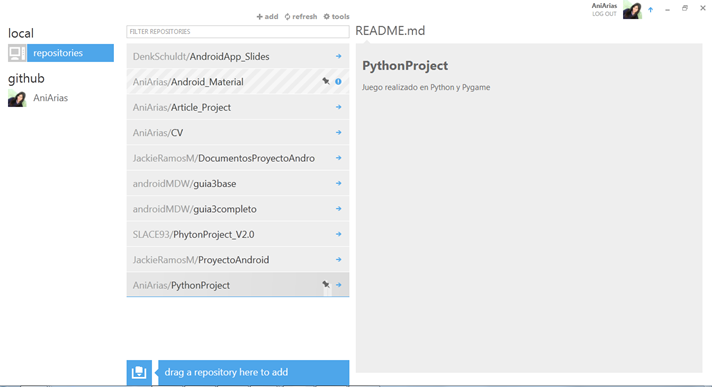
\includegraphics[width=0.8\textwidth]{imagenes_usuario/git2.png}
\newline
\newline
		\endgroup
	\end{center}

	\begin{center}
		\begingroup
			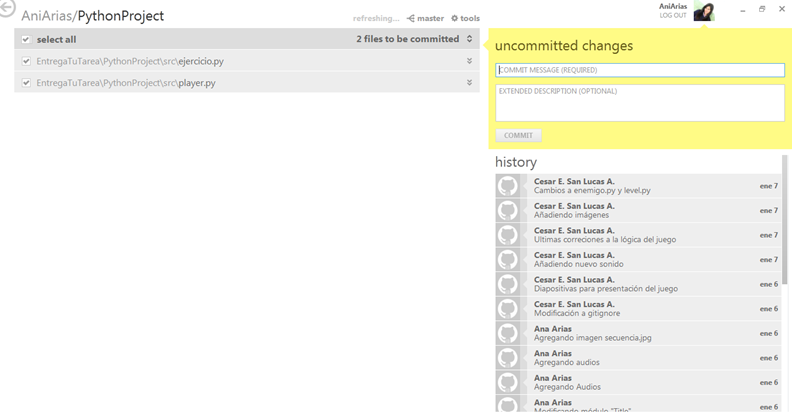
\includegraphics[width=0.8\textwidth]{imagenes_usuario/git3.png}
\newline
\newline
		\endgroup
	\end{center}

La interfaz de Github permite realizar commits de manera mucho mas rápida y mas detallada; me pareció mu interesante la rapidez con que se actualizaban los proyectos cada vez que se modificaba algo.
Recomendaría utilizar la interfaz de GitHub para las personas que recién empiecen a utilizar esta herramienta.
\newline
\newline
Seguiré utilizandola para futuros proyectos y en mi vida profesional.

 \ref{capitulouno}


%---------------------------------------------------------------------------------------------------------------------------------
%--------------------------------------------------------------LATEX------------------------------------------------------
%---------------------------------------------------------------------------------------------------------------------------------


\chapter{Herramienta LateX\label{capitulouno}}

	\begin{center}
		\begingroup
			
\includegraphics[width=0.27\textwidth]{imagenes_usuario/latex.jpg}
		\endgroup
	\end{center}


	\begingroup
		\large{
			\textbf{
				Experiencias y Anécdotas: LaTeX
				\newline
				\newline
			}
		}
	\endgroup

Latex es una buena opción al momento de la creación de documentos de distinto tipo, una herramienta que nos saca de la rutina de los mismos editores de texto que utilizamos a diario; y sin embargo Latex ofrece las mismas características que dichos editores.
\newline	
\newline	
Latex  a pesar de aparentar dificultad, es una herramienta sencilla de utilizar, solo es cuestión de conocer los comandos que permiten editar el formato de nuestro documento.
Otra ventaja de Latex es que existen plantillas para realizar distintos tipos de documentos, estas plantillas facilitan la edición del formato de un texto que quizás no sepamos cómo debería estar formado.
\newline	
\newline	
Como conclusión, el uso de esta herramienta me pareció entretenida y útil, además, fue un reto ya que como programadores debemos ser capaces de adaptarnos a cualquier herramienta.
\newline
\newline		
Existen muchos tutoriales de cómo utilizar Latex, los cuales fueron de mucha ayuda al momento de generar el primer documento que fue el CV, ya que al ser una herramienta nueva, tuve que introducirme al uso de ésta y cuáles son las mejores cualidades que ofrece; para este artículo tengo más experiencia y me costó menos tiempo hacerlo y se me hizo mucho más entretenido.
\newline
Nuestra primera tarea en Latex fue el Curriculum Vitae, al principio el uso de latex, al ser algo nuevo para mi, fue un poco tedioso sin embargo en internet se encuentran muchos tutoriales para crear simpaticos documentos de distintos tipos; se encuentran un sin fin de plantillas que ayudan a empezar a aprender a programar y decorar mucho mejor los documentos que queramos realizar.
Con el tiempo cada vez se hizo mas fácil su uso.
\newline
Lo que me causó mas problema con esta herramienta eran los paquetes que se tenian que instalar para hacer funcionar algunas plantillas, ya que la instalación de estos paquetes a veces era muy rápida y otras veces muy lenta.

La realizacion de mi Curriculum Vitae fue muy útil, ya que éste me ha servido ya en múltiples ocasiones.

El uso de Latex no es cosa del otro mundo, sin embargo existen muchos comandos que sirven para dar formato a nuestros documentos, debemos utilizarlos correctamente ya que si nos olvidamos de cerrar algún bloque de texto o una sentencia, nuestro programa no se compliará de manera exitosa.
\newline
\newline
\newline
\newline
\newline
\newline
\newline
\newline
\newline
\newline
\newline
\newline
\newline
\newline
\newline
\newline
\newline
\newline
\newline
\newline
\newline
\newline
\newline
\newline
\newline
\newline
\newline
\newline

 \ref{capitulouno}















\end{document}